\documentclass{note}
\addtolength{\topmargin}{-2cm}
\addtolength{\textheight}{2.2cm}
\usepackage{mathptm,mydef,myenv}
\usepackage[all]{xy}
%\usepackage{MinionPro}
\usepackage{courier}
\usepackage{alltt}
\usepackage[T1]{fontenc}
\usepackage{graphicx}
\DeclareGraphicsExtensions{.png,.jpg}


\usepackage{hyperref}
\hypersetup{
    colorlinks, 
    citecolor=black, 
    filecolor=black, 
    linkcolor=blue, 
    urlcolor=black
}

\begin{document}
\small

\begin{center}
{\large\bf \textcolor{blue2}{Notes on Unix V6 for X86}}
\end{center}

\vspace*{1cm}

\tableofcontents
\pagebreak

\section{Introduction}

\subsection{Problem statement}
\bit
\w \bb{What we want to do}:
  \bit
  \w Multiple jobs (abtract notion) to do (OPTIONAL: owned by multiple users)
  \w Jobs are given in the form of a ``\bb{program}'' (in any possible form --
  e.g. in a disk)
  \eit
\w \bb{What we are given}:
  \bit
  \w von-Neumann, stored-program machine (processor, memory, I/O)
  \eit
\w \bb{Constraints}:
  \bit
  \w Protection: program executions should be protected from each other; also,
  kernel should be protected from program exeuctions
  \w No deadlock, etc.
  \eit
\eit

\subsection{Solution: OS}
\bit
\w \textcolor{red2}{\bf TAPPING (DOWNWARD)}: HW (processor + devices + console + etc.) is just an \textcolor{red2}{\em
  autonomous, free-running pieces of metal\/}.  
  \bit
  \w Suppose you want to ``use'' these pieces of metal. Then, you need to add a
``tap'' to this free-running wheel, through which you do something useful.
  OS allows that. 
  \w ``Stored program concept'' already adds one level of abstraction (compare
  this to a circuitry which performs a single fixed-function).
  \w \bb{WHAT MACHINE CAN DO}:
     \bit
     \w If you put instruction on memory location and set EIP to that
     location,
       the machine will execute it automatically.
     \eit
  \w \bb{WHAT TO DO TO USE THE MACHINE}:
     \bit
     \w Put (well-planned) instructions on memory and set EIP.
     \w determine the meaning of ``well-planned instructions''
     \w Now, the notion of ``program'' comes in and
     program-to-machine-instruction mapping comes to play.
     \eit
  \eit
\w \textcolor{red2}{\bf INTERFACE (UPWARD)}: OS provides ``services'' to user programs through an \bb{interface}.
   \bit
   \w interfaces must be \textcolor{red2}{simple and narrow}
   \w but users want many sophisticated features
   \w HOW TO RECONCILE THESE CONFLICTING NEEDS:
     \bit
     \w select a good set of small interfaces which can be \bb{combined} to
     support any sophisticated feature
     \w find a \bb{basis} set from which every thing can be combined
         ({\em efficiently\/})
     \eit
   \eit

\w \textcolor{red2}{\bf{}YET ANOTHER PROGRAM}: An OS is yet another
program. Just like an interpreter is yet another program. 
   \bit
   \w Consider a simple example -- uniprocessor, single-threaded system.
   \w \textcolor{red2}{From HW viewpoint, there is only one program running --
     a program named ``kernel''.}
   \w Kernel allows multiple processes to ``share'' HW through
   \textcolor{red2}{\bf multiplexing}. 
     \bit
     \w SHARE $\equiv$ MULTIPLEX
     \eit
   \w that is, it gives an illusion that that multiple processes are running
   (multiprogramming) even if actually a single program called ``kernel'' is
   running 
   \eit
\w \textcolor{red2}{\bf{}SYSTEM CALLS}
  \bit
  \w processes: fork, exit, wait, kill, sbrk, sleep, getpid
  \w files: ope, read, write, close, dup, mkdir, chdir, mknod, fstat, link,
  unlink
  \eit
\w \textcolor{red2}{\bf SHELL}
  \bit
  \w \bb{THOUGHT EXPERIMENT}: trace in your brain how a shell is implemented
  on Unix 
  \w it has all essentials -- process creation, deletion, resource allocation,
  etc. 
  \w provides the interaction between USERs and MACHINES (via OS)
  \eit
\eit

\subsection{x86 calling convention}
\bit
\w \textcolor{red2}{\bb{HARDWARE}} (x86) provides \bb{stack registers} (\verb+%esp+, \verb+%ebp+), and \bb{stack instructions} (\verb+push+, \verb+pop+, \verb+call+, verb+ret+)
  \begin{alltt}
   EXAMPLE INSTRUCTION    WHAT IT EFFECTIVELY DOES
   -------------------    ------------------------
   \textcolor{blue2}{pushl %eax}             subl $4, %esp         ; stack grows down
                          movl %eax, (%esp)
   \textcolor{blue2}{popl %eax}              movl (%esp), %eax
                          addl $4, %esp
   \textcolor{blue2}{call 0x12345}           pushl %eip
                          movl $0x12345, %eip
   \textcolor{blue2}{ret}                    popl %eip 
  \end{alltt}


\w \textcolor{red2}{\bb{COMPILER}} (GCC) dictates how the stack is
used. Contract between caller and callee on x86:
  \bit
  \w \bb{at entry to a function} (i.e. right after
  \textcolor{red2}{\textbf{\texttt{call}}}} instruction is executed)
     \bit
     \w \verb+%eip+ points at first instruction of function  ({\tt{}call}
              pushes \verb+%eip+ which is the \bb{return address})
     \w \verb+%esp+4+ points at first argument
     \w \verb+%esp+ points at return address 
     \eit
  \w \bb{right after \textcolor{red2}{\textbf{\texttt{ret}}} instruction is executed}
     \bit
     \w \verb+%eip+ contains return address
     \w \verb+%esp+ points at arguments pushed by caller
     \w CALLEE may have trashed arguments
     \w \verb+%eax+ (and \verb+%edx+, if return type is 64-bit) contains
              return value (or trash if function is void) 
     \w \bb{caller-saved registers} (\verb+%eax+, \verb+%edx+ (above), and
                                \verb+%ecx+) may be trashed during the
                                ``call'' 
       \bit
       \w so, in case caller have been using these registers, caller should save
          it (and restore it later before it will use it again)
       \w COMPILER must insert save/restore code in CALLER-side
       \eit
     \w \bb{callee-saved registers} (\verb+%ebp+, \verb+%ebx+, \verb+%esi+, \verb+%edi+) must contain contents
     from time of \bb{\texttt{call}} 
        \bit
        \w i.e. callee should have properly restored these registers to contain
        pre-call values
       \w COMPILER must insert save/restore code in CALLEE-side
        \eit
     \eit
  \eit
\w Functions can do anything that doesn't violate contract. By convention, GCC
does more: 
  \bit
  \w each function has a stack frame marked by \verb+%ebp+, \verb+%esp+
\begin{alltt}
		       +------------+   |
		       | arg 2      |   \textbackslash
		       +------------+    >- previous function's stack frame
		       | arg 1      |   /
		       +------------+   |
		       | ret %eip   |   /  <= "CALL" pushed %eip
		       \textcolor{red2}{+============+}
		       | saved %ebp |   \textbackslash  <= by "push %ebp" inside callee
		%ebp-> +------------+   |  <= by "move %esp, %ebp" in callee
		       |            |   |
		       |   local    |   \textbackslash
		       | variables, |    >- current function's stack frame
		       |    etc.    |   /
		       |            |   |
		       |            |   |
		%esp-> +------------+   /  <= by "stack alloc" in callee
   \end{alltt}
    \w \verb+%esp+ can move to make stack frame bigger, smaller
    \w \verb+%ebp+ points at saved \verb+%ebp+ from previous function, chain
             to walk stack 
    \w \textcolor{red2}{\bb{function prologue}}: CALLEE performs upon entry
     \begin{verbatim}
    			pushl %ebp        ; push curr %ebp (%esp increments)
                                          ; 
    			movl %esp, %ebp
     \end{verbatim}
     \w textcolor{red2}{\bb{}function init setup}: CALLEE prepares function
       execution; allows local vars, set current stackframe
    		
     \w \textcolor{red2}{\bb{}function epilogue}: CALLEE performs upon exit
     \begin{verbatim}
                        // can easily find return EIP on stack:
    			movl %ebp, %esp
    			popl %ebp
     \end{verbatim}
     \eit
\eit



\pagebreak
\section{The First Process}
\subsection{Boot process}
\xymatrix@-0.7pc{
  *+[F]\txt<3cm>{\bb{\textcolor{blue2}{BIOS at 0xffff0}}} \ar[r] &
     *+[F]\txt<3cm>{setup IVT}\ar[d]  & \bullet  \ar[r]&
     *+[F]\txt<3cm>{\bb{\textcolor{blue2}{Boot sector at 0x07c00}}}  \ar[r]& 
     *+[F]\txt<3cm>{\bb{.globl start}} \ar[d]\\
    & *+[F]\txt<3cm>{init devices \\ (e.g. display)}\ar[d] &&
    & *+[F]\txt<3cm>{disable interrupts (cli) } \ar[d]
   \\
    & *+[F]\txt<3cm>{init PCI bus} \ar[d]&&
    & *+[F]\txt<3cm>{zero out {\tt{}\%ds,\%es,\%ss}} \ar[d]
   \\
    & *+[F]\txt<3cm>{search for ``bootable'' devices} \ar[d]&&
    & *+[F]\txt<3cm>{enable A20 addr line} \ar[d]
   \\
    & *+[F]\txt<3cm>{load \bb{boot sector} into 0x07c00} \ar[d]&&
    & *+[F]\txt<3cm>{switch from real to protected mode} \ar[d]
   \\
    & *+[F]\txt<3cm>{transfer control to 0x7c00} \ar[r]& \bullet \ar[uuuuu]&
    & *+[F]\txt<3cm>{ljmp 0x0008:\$start32} \ar[d]
   \\
   &&&&*+[F]\txt<3cm>{load segment regs from kernel data + stack} \ar[d]
   \\
   \bullet\ar[d] &&&&*+[F]\txt<3cm>{call \textcolor{red2}{\bb{bootmain}}} \ar[llll]
   \\
  *+[F]\txt<3cm>{\bb{\textcolor{blue2}{bootmain:}}} \ar[r] & *+[F]\txt<3cm>{read ELF header
  }\ar[d]
  \\
 & *+[F]\txt<3cm>{read segments to \bb{ph.p\_pa}} \ar[d] 
  \\
 & *+[F]\txt<3cm>{call \bb{ELFHDR.e\_entry()}} \ar@{~>}[rrr] &&&
*+[F]\txt<3cm>{\textcolor{red2}{\bb{KERNEL (entry.S)}}}
}

\vspace*{0.2cm}

\pagebreak

\subsection{Kernel entry (entry.S)}

\vspace*{0.2cm}

\xymatrix@-0.7pc{
*+[F]\txt<3cm>{\textcolor{blue2}{\bb{entry.S at 0x100000:}}} \ar[r] &
*+[F]\txt<11cm>{\textcolor{red2}{setup pgdir s.t. va [KERNBASE, KERBASE+4MB) is mapped to pa [0,4MB)}} \ar[d] 
\\
& *+[F]\txt<11cm>{clear frame pointer reg (EBP) from stack trace} \ar[d]
\\
& *+[F]\txt<11cm>{set stack pointer (ESP) to \bb{\$(bootstacktop)}} \ar[d]
\\
& *+[F]\txt<11cm>{call \textcolor{red2}{\bb{i386\_init}}}
}

\vspace*{0.8cm}

\bit
\w Entry sequence:
\begin{alltt}
  .globl entry
  entry:
    # Turn on page size extension for 4Mbyte pages
    movl    %cr4, %eax
    orl     $(CR4_PSE), %eax
    movl    %eax, %cr4
    # Set page directory
    movl    $(\textcolor{blue2}{\textbf{V2P_WO}}(\textcolor{red2}{\textbf{entrypgdir}})), %eax
    movl    %eax, %cr3
    # Turn on paging.
    movl    %cr0, %eax
    orl     $(CR0_PG|CR0_WP), %eax
    movl    %eax, %cr0

    # \textbf{Set up the stack pointer.}
    movl $(\textcolor{red2}{\textbf{stack}} + KSTACKSIZE), \textcolor{red2}{\textbf{%esp}}

    # \textbf{Jump to main()}, and switch to executing at
    # high addresses. The indirect call is needed because
    # the assembler produces a PC-relative instruction
    # for a direct jump.
    mov $main, %eax
    jmp *%eax

  .comm \textcolor{red2}{\textbf{stack}}, KSTACKSIZE
\end{alltt}
\w Entry page table is defined in \textbf{main.c}.
\begin{alltt}
  // Boot page table used in entry.S and entryother.S.
  // Page directories (and page tables), must start on a page boundary,
  // hence the "__aligned__" attribute.  
  // Use PTE_PS in page directory entry to enable 4Mbyte pages.
  __attribute__((__aligned__(PGSIZE)))
  \textcolor{red2}{\textbf{pde_t entrypgdir[NPDENTRIES]}} = \{
    // Map VA's [0, 4MB) to PA's [0, 4MB)
    [0] = (0) | PTE_P | PTE_W | PTE_PS,
    // Map VA's [KERNBASE, KERNBASE+4MB) to PA's [0, 4MB)
    [KERNBASE>>PDXSHIFT] = (0) | PTE_P | PTE_W | PTE_PS,
  \};
\end{alltt}
\eit
\vspace*{0.7cm}

\pagebreak
\subsection{Kernel init (kern/init.c)}

\xymatrix@-0.5pc{
*+[F]\txt<3cm>{\textcolor{blue2}{\bb{i386\_init:}}} \ar[r] &
   *+[F]\txt<3cm>{cons\_init} \ar[dd]\ar[r] & *+[F]\txt<3cm>{cga\_init} \ar[d]
\\
 & & *+[F]\txt<3cm>{kbd\_init} \ar[d]
\\
 & *+[F]\txt<3cm>{test\_backtrace}  \ar[d] & *+[F]\txt<3cm>{serial\_init} 
\\
 &  *+[F]\txt<3cm>{monitor}
\\
}

\vspace*{0.8cm}

\subsection{Console (kern/console.c)}

\xymatrix@-0.5pc{
*+[F]\txt<3cm>{\bb{getchar:}} \ar[r] &
  *+[F]\txt<3cm>{cons\_getc}   \ar[r] &
  *+[F]\txt<3cm>{serial\_intr}   \ar[r] \ar[d]&
  *+[F]\txt<4cm>{cons\_instr(serial\_proc\_data)} 
\\
&&  *+[F]\txt<3cm>{kbd\_intr}   \ar[r] &
  *+[F]\txt<4cm>{cons\_instr(kbd\_proc\_data)} 
\\
*+[F]\txt<3cm>{\bb{cputchar:}} \ar[r] &
  *+[F]\txt<3cm>{cons\_putc}   \ar[r] &
  *+[F]\txt<3cm>{serial\_putc}   \ar[d]
\\
  &&*+[F]\txt<3cm>{lpt\_putc}   \ar[d]
\\
&&  *+[F]\txt<3cm>{cga\_putc}
}


\subsection{Monitor (kern/monitor.c)}

\xymatrix@-0.5pc{
*+[F]\txt<3cm>{\bb{monitor:}} \ar[r] &
  *+[F]\txt<3cm>{readline} \ar[d]  \ar[r] &
  *+[F]\txt<3cm>{getchar}   \ar[r] \ar[d]&
  *+[F]\txt<3cm>{cons\_getc} 
\\
 &
  *+[F]\txt<3cm>{runcmd}    &
  *+[F]\txt<3cm>{\bb{cprintf}}   \ar[r] \ar[d]&
  *+[F]\txt<3cm>{vcprintf} 
\\
 &
&
  *+[F]\txt<3cm>{cputchar}   \ar[r]&
  *+[F]\txt<3cm>{cons\_putc} 
}

\subsection{Printfmt (lib/printfmtc)}

\xymatrix@-0.5pc{
*+[F]\txt<3cm>{\bb{cprintf:}} \ar[r] &
  *+[F]\txt<3cm>{vcprintf}   \ar[r] &
  *+[F]\txt<3cm>{vcprintfmt}   \ar[r] &
  *+[F]\txt<3cm>{putch} \ar[d]
\\
  *+[F]\txt<3cm>{\bb{printfmt:}} \ar@/_4ex/[rru]   &&
 &
  *+[F]\txt<3cm>{cputchar} 
}

\pagebreak
\subsection{proc: Per-process state}
\begin{alltt}
  \textcolor{red2}{\textbf{struct proc}} \{
    uint sz;                     // Size of process memory (bytes)
    pde_t* \textbf{pgdir};                // Page table
    char *\textbf{kstack};                // Bottom of kernel stack for this process
    enum procstate \textbf{state};        // State: running, ready, waiting for I/O, exiting
    volatile int pid;            // Process ID
    struct proc *parent;         // Parent process
    struct trapframe *\textbf{tf};        // Trap frame for current syscall
    struct context *context;     // swtch() here to run process
    void *chan;                  // If non-zero, sleeping on chan
    int killed;                  // If non-zero, have been killed
    struct file *ofile[NOFILE];  // Open files
    struct inode *cwd;           // Current directory
    char name[16];               // Process name (debugging)
  \};

  // saved registers for kernel context switches
  \textcolor{red2}{\textbf{struct context}} \{
    uint edi;
    uint esi;
    uint ebx;
    uint ebp;
    uint eip;
  \};

  // Per-CPU state
  \textcolor{red2}{\textbf{struct cpu}} \{
    uchar id;                    // Local APIC ID; index into cpus[] below
    struct context *\textbf{scheduler};   // swtch() here to enter scheduler
    struct taskstate ts;         // Used by x86 to find stack for interrupt
    struct segdesc gdt[NSEGS];   // x86 global descriptor table
    volatile uint started;       // Has the CPU started?
    int ncli;                    // Depth of pushcli nesting.
    int intena;                  // Were interrupts enabled before pushcli?
  
    // CPU-local storage variables; see below
    struct cpu *cpu;
    struct proc *\textbf{proc};           // The currently-running process.
  \};
\end{alltt}

\subsection{Creating the first user process (main.c $\ra$ proc.c)}

\xymatrix@-0.5pc{
*+[F]\txt<3cm>{\textcolor{blue2}{\bb{userinit:}}} \ar[r]& 
    *+[F]\txt<5cm>{p = \textcolor{red2}{\bb{allocproc()}}} \ar[ddddddd]\ar[r]  &
    *+[F]\txt<5cm>{search PTABLE for UNUSED}  \ar[d]
   \\
  &&
    *+[F]\txt<5cm>{p.state = {\tt{}EMBRYO}}  \ar[d]
  \\
  &&
    *+[F]\txt<5cm>{p.kstack = \bb{kalloc()}} \ar[d]
   \\
  &&
    *+[F]\txt<5cm>{// allocate kernel stack\\
     sp = p.kstack + {\tt{}KSTACKSIZE} (4096)}  \ar[d]
  \\
  &&
    *+[F]\txt<5cm>{// allocate trapframe in stack\\
            sp -= sizeof(trapframe); \\\bb{p.tf} = (trapframe *) sp}
    \ar[d] 
  \\
  &&
    *+[F]\txt<5cm>{// allocate context in stack\\
      sp -= sizeof(context); \\\bb{p.context} = (context *) sp}
    \ar[d] 
  \\
  &&
    *+[F]\txt<5cm>{// set \bb{forkret} as the\\ // ``context'' to return to\\
           \bb{p.context.eip = (uint) forkret}}
  \\
  &
    *+[F]\txt<5cm>{// alloc kernel VM (set pgtable)\\p.pgdir =
      \bb{\textcolor{red2}{setupkvm()}}} \ar[dd] \ar[r]
   & 
    *+[F]\txt<5cm>{pgdir = (pde\_t*) \bb{kalloc()}} \ar[d]
   \\
   && 
    *+[F]\txt<5cm>{\bb{mappage}(pgdir, k.virt, k.phy\_sz, k.phy\_start)}
   \\
\txt<5cm>{{\tt{}\_binary\_initcode\_start} points to compiled binary of
  \bb{initcode.S}} \ar@{.>}[r]&    *+[F]\txt<5cm>{\textcolor{red2}{\bb{inituvm}}(p.pgdir, {\tt{}\_binary\_initcode\_start},
   {\tt{}\_binary\_initcode\_start})} \ar[r]\ar[dd]
   &
    *+[F]\txt<5cm>{mem = \bb{kalloc()}} \ar[d]
   \\
   &&
    *+[F]\txt<5cm>{\bb{mappage}(pgdir, 0, PGSIZE, \bb{V2P(mem)}, PTE\_U)}
   \\
& *+[F]\txt<5cm>{fill in p.tf (trapframe)} \ar[d]
  \\
& *+[F]\txt<5cm>{p.cwd = \bb{namei}(``/'')} \ar[d]
  \\
& *+[F]\txt<5cm>{p.state = {\tt{}RUNNABLE}}
}

\pagebreak

\bit
\w \bb{allocproc} sets up the new process with a specially prepared kernel
stack and set of kernel registers thta cause it \textcolor{red}{to ``return''
  to user space when it first runs}
\begin{alltt}
\textcolor{red2}{\textbf{static struct proc *allocproc(void)}}
\{
  struct proc *p;
  char *sp;

  acquire(&ptable.lock);
  for(p = ptable.proc; p < &ptable.proc[NPROC]; p++)
    if(p->state == UNUSED)
      goto found;
  release(&ptable.lock);
  return 0;

found:
  p->state = EMBRYO;  p->pid = nextpid++;
  release(&ptable.lock);

  // Allocate kernel stack.
  if((p->kstack = kalloc()) == 0) \{
    p->state = UNUSED;
    return 0;
  \}
  sp = p->kstack + KSTACKSIZE;
  
  // Leave room for trap frame.
  sp -= sizeof *p->tf;
  p->tf = (struct trapframe*)sp;
  
  // Set up new context to start executing at \textbf{forkret},
  // which returns to \textbf{trapret}.
  sp -= 4;
  *(uint*)sp = (uint)\textcolor{red2}{\textbf{trapret}};

  sp -= sizeof *p->context;
  p->context = (struct context*)sp;
  memset(p->context, 0, sizeof *p->context);
  \textcolor{red2}{\textbf{p->context->eip = (uint)forkret;}}
  return p;
\}

// A fork child's very first scheduling by \textbf{scheduler()} will swtch 
// here.  \textbf{"Return" to user space.}
\textcolor{red2}{\textbf{void forkret(void)}}
\{
  static int first = 1;
  // Still holding ptable.lock from scheduler.
  release(&ptable.lock);
  if (first) \{
    // Some initialization functions must be run in the context
    // of a regular process (e.g., they call sleep), and thus cannot 
    // be run from main().
    first = 0; initlog();
  \}
  // Return to "caller", actually \textbf{trapret} (see allocproc).
\}

.globl trapret
\textcolor{red2}{\textbf{trapret}}:
  // pop EAX,EBX,ECX,EDX,ESP,EBP,ESI,EDI 
  // (as in bottom 8-words of trapframe)
  \textcolor{red2}{\textbf{popal}}
  popl %gs
  popl %fs
  popl %es
  popl %ds
  addl $0x8, %esp # trapno and errcode
  iret
\end{alltt}

\eit

\paragraph{So, what happens when {\bf \texttt{fork}} executed?}
  \ben
  \w user code invokes system call \bb{fork} (\verb+int $T_SYSCALL+)
  \w now in kernel space
  \w \bb{fork} calls \bb{allocproc}
  \w \bb{allocproc} will set up kernel stack (see Figure~1-3)
     \bit
     \w will prepare two things: \bb{forkret} and \bb{trapret} 
     \w \bb{forkret}: let \verb+p->context.eip+ point to address of function
     \verb+forkret+
     \w so, when \verb+swtch(context **old, context*new)+ is executed, it will context switch to a user
     function \bb{forkret} 
     \w \bb{forkret} will be a typical function and its \bb{return} will look
     at the stack return address -- which is \bb{trapret}
     \w so, after return from \bb{forkret}, \bb{trapret} code (assembly code
     defined in \verb+vectors.S+ will be executed
     \w \bb{trapret}: restores user registers from values stored at the top of
     the kernel stack and jumps into the process
     \eit
  \een

\paragraph{First process vs. oridinary {\bf \texttt{fork}}}
\bit
\w When setting trapframe in kernel stack,
  \bit
  \w first process: set EIP to user-space location 0
  \w oridinary stack: set EIP to the instruction right after fork
  \eit
\eit

\subsection{Running the first process}
\xymatrix@-0.5pc{
*+[F]\txt<3cm>{\bb{main}} \ar[r]& 
    *+[F]\txt<3cm>{\bb{userinit}} \ar[r]\ar[d] & 
    *+[F]\txt<6cm>{create the first process (\bb{initcode.S}) at 0x0} 
   \\
& 
  *+[F]\txt<3cm>{\bb{mpmain}}  \ar[r] &
    *+[F]\txt<6cm>{\bb{idtinit}: load idt register} \ar[d] 
\\
&&  *+[F]\txt<6cm>{xchg(\&cpu.started, 1): tell startothers() we're up} \ar[d] 
\\
\bullet \ar[dd]&&  *+[F]\txt<6cm>{call \textcolor{red2}{\bb{scheduler}}} \ar[ll] 
\\
\\
*+[F]\txt<3cm>{\textcolor{blue2}{\bb{scheduler:}}} \ar[r] 
  & *+[F]\txt<4cm>{enable interrupts (sti)} \ar[d]
\\
\bullet\ar[ru]  & *+[F]\txt<4cm>{acquire(\&PTABLE.lock)} \ar[d]
\\
  & *+[F]\txt<4cm>{pick a RUNNABLE process, p} \ar[d]
\\
  & *+[F]\txt<4cm>{\textcolor{red2}{\bb{switchuvm(p)}}} \ar[d] \ar[r]
 & *+[F]\txt<6cm>{switch TSS and HW page table to p}
\\
  & *+[F]\txt<4cm>{p.state = {\tt{}RUNNING}} \ar[d]
\\
  & *+[F]\txt<4cm>{\textcolor{red2}{\bb{switch}}(\&cpu.scheduler, p.context)} \ar[d] \ar[r] &
*+[F]\txt<6cm>{{\em save current register context in OLD (L) and load register
  context from NEW (R)\/}}
\\
  & *+[F]\txt<4cm>{\textcolor{red2}{\bb{switchkvm}}} \ar[d] \ar[r] &
*+[F]\txt<6cm>{//switch to the kernel page table \\ \bb{lcr3(V2P(kpgdir))}}
\\
 \bullet\ar[uuuuuu] & *+[F]\txt<4cm>{release(\&PTABLE.lock)} \ar[l]
\\
}

\pagebreak
\subsection{Context switch (switch.S)}
\begin{alltt}
  # Context switch
  #
  #   \textcolor{red2}{\textbf{void swtch(struct context **old, struct context *new);}}
  #
  # Save current register context in old
  # and then load register context from new.

  .globl swtch
  swtch:
    movl 4(%esp), %eax
    movl 8(%esp), %edx

    # Save old callee-save registers
    pushl %ebp
    pushl %ebx
    pushl %esi
    pushl %edi

    # Switch stacks
    movl %esp, (%eax)
    movl %edx, %esp

    # Load new callee-save registers
    popl %edi
    popl %esi
    popl %ebx
    popl %ebp
    ret
\end{alltt}

\vspace*{0.5cm}

\subsection{The first system call: exec}

\xymatrix@-0.5pc{
*+[F]\txt<4cm>{\textcolor{blue2}{First process (\bb{initcode.S})}} \ar[r] & 
   *+[F]\txt<4cm>{pushl \$argv} \ar[d]\\
& 
   *+[F]\txt<4cm>{pushl \$init} \ar[d]\\
& 
   *+[F]\txt<4cm>{pushl 0 /* PC */} \ar[d]\\
& 
   *+[F]\txt<4cm>{move \textbf{\$SYS\_exec}, \%eax} \ar[d]\\
& 
   *+[F]\txt<4cm>{\textcolor{red2}{\bf{}int \$T\_SYSCALL}} & \txt<4cm>{ask kernel to run {\tt{}exec}
     syscall} \ar@{.}[l] \ar@{.>}@/_10ex/[luuu]_{\txt{execute program named {\tt init}}}\\
}

\pagebreak
\section{Virtual Memory}
\subsection{Basics}
\bit
\w \bb{VIRTUAL MEMORY}: every xv6 process has an illusion that it has \textbf{its own address
  space}.
\w x86 uses \bb{paging} to implement virtual memory.
\w paging is technically implemented by managing
\textcolor{red2}{\bb{per-process page tables}} -- i.e. set up page tages for
each process
\w \bb{What HW provides for paging}
   \bit
   \w page directory register
   \eit
\w \bb{What SW (OS) needs to provide for paging}:
   \bit
   \w 
   \eit
\eit
\subsection{Setting up kernel virtual memory}
\xymatrix@-0.5pc{
*+[F]\txt<3cm>{\textcolor{blue2}{\bb{main:}}} \ar[r] & 
  *+[F]\txt<4cm>{\textcolor{red2}{\bb{kinit}}(end, P2V(4MB)}  \ar[d]\ar[r] &
   *+[F]\txt<7cm>{phys page allocation}
  \\
 & *+[F]\txt<4cm>{\bb{kvmalloc}} \ar[r] &
    *+[F]\txt<7cm>{kpgdir = \bb{setupkvm()}}  \ar[d]
  \\
 & &
    *+[F]\txt<7cm>{\bb{switchkvm()}} 
\\
*+[F]\txt<3cm>{\textcolor{blue2}{\bb{setupkvm:}}} \ar[r] &
  *+[F]\txt<4cm>{pde\_t pgdir = \bb{kalloc()}} \ar[d] 
 \\
&
  *+[F]\txt<4cm>{memset(pgdir, 0, {PGSIZE})}  \ar[d]
 \\
& 
  *+[F]\txt<4cm>{foreach \textcolor{red2}{\bb{kmap}} entry} \ar[r] &
  *+[F]\txt<7cm>{\textcolor{red2}{\bb{mappages}}(pgdir, k.virt, (k.phys\_end - k.phys\_start),\\
                          (uint) k.phys\_start, k.perm)}
}

\vspace*{0.5cm}

There is one page table per process, plus one that's used when
a CPU is not running any process ({\bb{kpgdir}). The kernel uses the
current process's page table during system calls and interrupts;
page protection bits prevent user code from using the kernel's
mappings.

\bb{setupkvm()} and \bb{exec()} set up every page table like this:
\bit
\w  \verb+[0,KERNBASE)+: user memory (text+data+stack+heap), 
                mapped to
                phys memory allocated by the kernel
\w \verb/[KERNBASE, KERNBASE+EXTMEM)/ mapped to \verb+[0, EXTMEM)+ 
    (for I/O space)
\w \verb/[KERNBASE+EXTMEM,data)/: mapped to \verb+[EXTMEM,V2P(data))+
                for the kernel's instructions and r/o data
\w \verb/[data, KERNBASE+PHYSTOP)/: mapped to \verb+[V2P(data), PHYSTOP)+,
                                  rw data + free physical memory
\w \verb+[0xfe000000,0)+: mapped direct (devices such as ioapic)
\eit
The kernel allocates physical memory for its heap and for user memory
between \verb+V2P(end)+ and the end of physical memory (\verb+PHYSTOP+)
(directly addressable from \verb/[end, P2V(PHYSTOP))/.
The following table defines the kernel's mappings, which are present in
 every process's page table.
\begin{alltt}
  \textcolor{red2}{\textbf{static struct kmap}} \{
    void *virt;
    uint phys_start;
    uint phys_end;
    int perm;
  \} kmap[] = \{
   \{ (void*)KERNBASE, 0,             EXTMEM,    PTE_W\}, // I/O space
   \{ (void*)KERNLINK, V2P(KERNLINK), V2P(data), 0\},     // kern text+rodata
   \{ (void*)data,     V2P(data),     PHYSTOP,   PTE_W\}, // kern data+memory
   \{ (void*)DEVSPACE, DEVSPACE,      0,         PTE_W\}, // more devices
  \};
\end{alltt}

\pagebreak

\subsection{Creating an address space by creating/populating page tables}
Creates PTEs for virtual addresses starting at \verb+va+ that refer to
physical addresses starting at \verb+pa+. \verb+va+ and \verb+size+ may not be
page-aligned.

\begin{alltt}
  \textcolor{red2}{\textbf{static int mappages(pde_t *pgdir, void *va, uint size, uint pa, int perm)}}
  \{
    char *a, *last;
    pte_t *pte;
  
    a = (char*) PGROUNDDOWN((uint) va);
    last = (char*) PGROUNDDOWN(((uint) va) + size - 1);
    for (;;) \{
      if ((pte = \textcolor{red2}{\textbf{walkpgdir}}(pgdir, a, 1)) == 0)
        return -1;
      if (*pte & PTE_P)
        panic("remap");
      *pte = pa | perm | PTE_P;
      if (a == last)
        break;
      a += PGSIZE;
      pa += PGSIZE;
    \}
    return 0;
  \}
\end{alltt}
The function \bb{walkpgdir} returns the address of the PTE in page table pgdir
that corresponds to virtual address va.  If alloc is not 0,  
create any required page table pages.
\begin{alltt}
  \textcolor{red2}{// A virtual address 'la' has a three-part structure as follows:
  // +--------10------+-------10-------+---------12----------+
  // | Page Directory |   Page Table   | Offset within Page  |
  // |      Index     |      Index     |                     |
  // +----------------+----------------+---------------------+
  //  \--- PDX(va) --/ \--- PTX(va) --/ }
  \textcolor{red2}{\textbf{static pte_t *walkpgdir(pde_t *pgdir, const void *va, int alloc)}}
  \{
    pde_t *pde;
    pte_t *pgtab;

    \textcolor{red2}{\textbf{pde = &pgdir[PDX(va)]}};
    if(*pde & PTE_P) \{
      \textcolor{red2}{\textbf{pgtab = (pte_t*) p2v(PTE_ADDR(*pde))}};
    \} 
    else \{
      if (!alloc || (\textcolor{red2}{\textbf{pgtab = (pte_t*) kalloc()}}) == 0)
        return 0;
      // Make sure all those PTE_P bits are zero.
      memset(pgtab, 0, PGSIZE);
      // The permissions here are overly generous, but they can
      // be further restricted by the permissions in the page table 
      // entries, if necessary.
      \textcolor{red2}{\textbf{*pde = V2P(pgtab) | PTE_P | PTE_W | PTE_U}};
    \}
    return \textcolor{red2}{\textbf{&pgtab[PTX(va)]}};
  \}
\end{alltt}

\pagebreak
\subsection{Paging in x86}
\bit
\w Since 10 bits for pgdir indices, there are 1024 pgdir's.
\w Each pgdir is a table of 1024 pgdir entries (i.e. 1024 pgtbls), where each
entry has 20 bits for PPN, and 12 bits for flags.
\w Each pgtbl points to 1024 entries, where each entry points to one page.
So, there are total 1024 $\times$ 1024 = 1M pages. 
\w One page is 4K (12 bit offset), so, 4GB addressable.
\eit

\subsection{Physical memory allocation}
\bit
\w all physical memory must be mapped (i.e. some page table should point to
each physical page). 
\w page table with these mapping involves allocating page-table pages.
\eit


\pagebreak
\subsection{System call: exec -- Creating user part of address space}\label{sec:sys_exec}
\xymatrix@-0.5pc{
  *+[F]\txt<4cm>{\textcolor{blue2}{\bb{exec(path, argv):}}} \ar[r] &
    *+[F]\txt<4cm>{ip = \textcolor{red2}{\bb{namei}}(path)} \ar[d] 
\\
  &  *+[F]\txt<4cm>{ilock(ip)} \ar[d] 
\\
  &  *+[F]\txt<4cm>{// read ELF header\\ \textcolor{red2}{\bb{readi}}(ip, \&elf, 0,
  sizeof(elf))} \ar[d] 
\\
  &  *+[F]\txt<4cm>{pgdir = \textcolor{red2}{\bb{setupkvm()}}} \ar[d]
\\
  &  *+[F]\txt<4cm>{//load program into memory;\\ for each prog sect header} \ar[ddd] \ar[r]&
   *+[F]\txt<7cm>{\bb{readi}(ip, \&ph, off, sizeof(ph)} \ar[d]
\\
&& *+[F]\txt<7cm>{\bb{allocuvm}(pgdir, sz, ph.vaddr+ph.memsz)} \ar[d]
\\
&& *+[F]\txt<7cm>{\bb{loaduvm}(pgdir, ph.vaddr, ip, ph.off, ph.filesz)}
\\
  &  *+[F]\txt<4cm>{iunlockput(ip)} \ar[d]
\\
  &  *+[F]\txt<4cm>{alloc two pages; first is inaccessible; second
  is user stack} \ar[d]\ar[r] & *+[F]\txt<7cm>{\bb{allocuvm}(pgdir, sz, sz +
  2*PGSIZE)} 
\\
  &  *+[F]\txt<4cm>{\textcolor{red2}{\bb{push args, prepare stack}}} \ar[d]
& 
\\
  &  *+[F]\txt<4cm>{save prog name for debugging} \ar[d] \ar[r]
& *+[F]\txt<7cm>{safestrcpy(proc.name, path, sizeof(proc->name)}
\\
  &  *+[F]\txt<4cm>{\textcolor{red2}{\bf{}commit to user image}} \ar[r] &
  *+[F]\txt<7cm>{oldpgdir = proc.pgdir} \ar[d]
\\
&&  *+[F]\txt<7cm>{{proc.pgdir = pgdir}} \ar[d]
\\
&&  *+[F]\txt<7cm>{{proc.tf.eip = elf.entry}} \ar[d]
\\
&&  *+[F]\txt<7cm>{{proc.tf.esp = sp}} \ar[d]
\\
&&  *+[F]\txt<7cm>{\bb{switchuvm}(proc)} \ar[d]
\\
&&  *+[F]\txt<7cm>{\bb{freevm}(oldpgdir)}
\\
})

\subsection{allocuvm: Allocating user memory}
\begin{alltt}
  \textcolor{red2}{// allocate page tables and physical memory to grow process
  // from oldsz to newsz, which need not be page aligned;
  // returns new size or 0 on error}
  \textcolor{red2}{\textbf{int allocuvm(pde_t *pgdir, uint oldsz, uint newsz)}}
  \{
    char *mem;
    uint a;

    // maximum process address space is [0, KERNBASE)
    if(newsz >= KERNBASE) return 0;
    if(newsz < oldsz) return oldsz;

    a = PGROUNDUP(oldsz);
    for (; a < newsz; a += PGSIZE) \{
      mem = kalloc();  // allocate one page from kmem.freelist
      if(mem == 0) \{
        cprintf("allocuvm out of memory");
        deallocuvm(pgdir, newsz, oldsz);
        return 0;
      \}
      memset(mem, 0, PGSIZE);
  
      \textcolor{red2}{\textbf{mappages}}(pgdir, (char*)a, PGSIZE, v2p(mem), PTE_W|PTE_U);
    \}
    return newsz;
  \}
\end{alltt}

\subsection{loaduvm: Loading user memory}
\begin{alltt}
\textcolor{red2}{  // Load a program segment into pgdir.  addr must be page-aligned
  // and the pages from addr to addr+sz must already be mapped.}
  \textcolor{red2}{\textbf{int loaduvm(pde_t *pgdir, char *addr, struct inode *ip, uint offset, uint sz)}}
  \{
    uint i, pa, n;
    pte_t *pte;

    if ((uint) addr \% PGSIZE != 0)
      panic("loaduvm: addr must be page aligned");
    for (i = 0; i < sz; i += PGSIZE) \{
      if ((pte = \textcolor{red2}{\textbf{walkpgdir}}(pgdir, addr+i, 0)) == 0)
        panic("loaduvm: address should exist");
      pa = PTE_ADDR(*pte);
      if (sz - i < PGSIZE)
        n = sz - i;
      else
        n = PGSIZE;
      if (readi(ip, p2v(pa), offset+i, n) != n)
        return -1;
    \}
    return 0;
  \}
\end{alltt}


\subsection{System call: exec -- Calling convention}

\pagebreak
\section{Traps, Interrupts, and Device Drivers}

\subsection{System calls, exceptions, and interrupts}

\vspace*{0.2cm}

\xymatrix@-0.5pc{
  *+[F]\txt<3cm>{processor}
  \ar[rrr]^{\txt{\textcolor{red2}{\textbf{exception}}}}_{\txt{\textcolor{black}{divzero,
        pgfault}}} &&& *+[F]\txt<3cm>{\textcolor{blue2}{\textbf{Unix V6}}} 
&&&   *+[F]\txt<3cm>{processor} 
\ar[lll]_{\txt{\textcolor{red2}{\textbf{system call}}}}^{\txt{\textcolor{black}{exec()}}}
\\ 
\\
&&&  *+[F]\txt<3cm>{device} \ar[uu]_{\txt{\textcolor{red2}{\textbf{interrupt}}}} \\
}

\vspace*{0.5cm}

\subsection{System call example: exec (initcode.S)}
\begin{alltt}
    # exec(init, argv)
    pushl $argv           // push arg on process's stack
    pushl $init           // 
    pushl $0              // where caller pc would be
    movl $SYS_exec, %eax  // put system call numuber, i.e.
                          // index to syscalls array, which 
                          // is a table of function ptrs
    int $T_SYSCALL        // generate "SYSCALL" trap
\end{alltt}
This interrupt (\verb+int $T_SYSCALL+) will eventually trigger the \verb+sys_exec+ function
shown in Section~\ref{sec:sys_exec}. 

\subsection{Assembly trap handlers}
\xymatrix@-0.5pc{
*+[F]\txt<3cm>{\textcolor{blue2}{\bb{main:}}} \ar[r] & 
  *+[F]\txt<4cm>{call \textcolor{red2}{\bb{tvinit}}}  \ar[r] &
   *+[F]\txt<8cm>{setup 256 entries of table \texttt{idt}} \ar[d]\\
& \txt<4cm>{\textcolor{red}{interrupt handler for interrupt {\em i} is at
       \texttt{vectors[i]}}} \ar@{.>}[r]& 
   *+[F]\txt<8cm>{\textcolor{red2}{\textbf{SETGATE}}(idt[i], 0, SEG\_KCODE <<
     3, vectors[i], 0);} \ar[d] \\
&&
   *+[F]\txt<8cm>{\textcolor{red2}{\textbf{SETGATE}}(idt[T\_SYSCALL], 1, SEG\_KCODE << 3, vectors[T\_SYSCALL], DPL\_USER);}
}

\subsection{Setting up interrupt gate descriptor}
\begin{alltt}
// Set up a normal interrupt/trap gate descriptor.
// - istrap: 1 for a trap (= exception) gate, 0 for an interrupt gate.
//   interrupt gate clears FL_IF, trap gate leaves FL_IF alone
// - sel: Code segment selector for interrupt/trap handler
// - off: Offset in code segment for interrupt/trap handler
// - dpl: Descriptor Privilege Level -
//        the privilege level required for software to invoke
//        this interrupt/trap gate explicitly using an int instruction.
\textcolor{red2}{\textbf{#define SETGATE(gate, istrap, sel, off, d)}} \{
  (gate).off_15_0 = (uint)(off) \& 0xffff;         
  (gate).cs = (sel);                               
  (gate).args = 0;                                 
  (gate).rsv1 = 0;                                 
  (gate).type = (istrap) ? STS_TG32 : STS_IG32;    
  (gate).s = 0;                                    
  (gate).dpl = (d);                                
  (gate).p = 1;                                    
  (gate).off_31_16 = (uint)(off) >> 16; \}
\end{alltt}

%% \bit
%% \item stack switch happens by setting up a TSS (task segment descriptor)
%%   through which the hardware loads a SSS (stack segment selector) and a new
%%   value of \verb+%esp+
%% \eit

%% \subsection{What happens on a interrupt/trap}
%% \ben
%% \w If the processor was executing in user mode
%%    \ben
%%    \w loads \verb+%esp+ and \verb+%ss+ from the task segment descriptor
%%    \w pushes the old \verb+%ss+ and \verb+%esp+ onto the new stack
%%    \een
%% \w If the processor was executing in kernel mode, none of above happens.
%% \w push \verb+%eflags+, \verb+%cs+, \verb+%eip+ registers
%% \w load \verb+%eip+ and \verb+%cs+ from the relevant IDT entry
   

%% \een
\subsection{What happens on system calls, exceptions, and interrupts}
\ben
\w \bb{put arguments}: put the arguments
\w \bb{interrupt generation -- \texttt{int} $n$}: 
    {\em \textcolor{red}{kernel and user-process (or device) are independent,
      autonomous entities;} so, for user-process to get service from kernel,
      it needs to tell them ``I need your help'' -- this is
      \textcolor{red}{interrupt generation}};

     from processor's viewpoint, interrupt is an
     \textcolor{red}{\textbf{asynchronous\/}} request
   \ben
   \w fetch $n$'s descriptor from the \bb{IDT (Interrupt Descriptor Table)},
   where $n$ is the argument of \verb+int+
   \w check priviledge level
   \w save \verb+%ss+ and \verb+%esp+ in CPU-internal registers
   \w load \verb+%ss+ and \verb+%esp+ from a task segment descriptor
   \w push \verb+%ss+, \verb+%esp+, \verb+%eflags+, \verb+%cs+, \verb+%eip+
   \w push \verb+%cs+ and \verb+%eip+ to the value in the descriptor
   \een
%\w \bb{stop normal processor loop}: on interrupt, notmal processor loop is
    stopped  (by H/W mechanism)
%\w \bb{save registers}: 
%    save the processor's registers for future transparent resume
%\w \bb{interrupt handler}: starts executing a new sequence called
%\textcolor{red}{interrupt handler}

\w \bb{get arguments}: the kernel must be able to retrieve ifnormation about
    the event (e.g. system call arguments)
\een

\subsection{IDT: Interrupt descriptor table}
IDT entries is setup  by an assembly code \verb+vectors.S+, which are
generated by the Perl script \verb+vectors.pl+.
\begin{alltt}
  # entry point to vector 0
  .globl vector0
  \textbf{vector0:}
    pushl $0      # 
    pushl $0      # trap no
    jmp alltraps
  # entry point to vector 1
  .globl vector1
  \textbf{vector1:}
    pushl $0
    pushl $1
    jmp alltraps
  ...
  \textbf{vector8:}
    pushl $8
    jmp alltraps
\end{alltt}

\subsection{trapasm.S}
\begin{alltt}
    # vectors.S sends all traps here.
  .globl alltraps
  alltraps:
    \textbf{# Build trap frame.}
    pushl %ds
    pushl %es
    pushl %fs
    pushl %gs
    pushal
  
    \textbf{# Set up data and per-cpu segments.}
    movw $(SEG_KDATA<<3), %ax
    movw %ax, %ds
    movw %ax, %es
    movw $(SEG_KCPU<<3), %ax
    movw %ax, %fs
    movw %ax, %gs

    \textbf{# Call trap(tf), where tf=%esp}
    pushl %esp
    call trap
    addl $4, %esp

    \textbf{# Return falls through to trapret...}
  .globl trapret
  trapret:
    popal
    popl %gs
    popl %fs
    popl %es
    popl %ds
    addl $0x8, %esp  # trapno and errcode
    iret
\end{alltt}
\subsection{Trapframes}
A trapframe (\verb+struct trapframe+) captures the contents of the processor
registers at the time of the trap. Actually, this structure ``interprets'' the
stack contents as a parameter. \textcolor{red2}{Some parts of the frame is
  filled up by the processor (according to the  calling convention), while
  others are filled up by \texttt{alltraps} code}. 

Typically, for a function call (i.e. ``jumping to new code''), when C-compiler
generated calling convention (pushing eip, return address, etc.) is enough,
you can just call them and let C-compiler generate code.
\textcolor{red2}{\em However, when it's not enough, you need to generate the code and mimic the
calling convention yourself in an assembly program. Trap handling is one of
such situation.}


\begin{alltt}
  // Layout of the trap frame built on the stack by the
  // hardware and by trapasm.S, and passed to trap().
  \textcolor{red2}{\textbf{struct trapframe}} \{
    // registers as pushed by \textbf{pusha}
    uint edi;
    uint esi;
    uint ebp;
    uint oesp;      // useless & ignored
    uint ebx;
    uint edx;
    uint ecx;
    uint eax;

    // rest of trap frame (pushed by alltraps)
    ushort gs;   ushort padding1;
    ushort fs;   ushort padding2;
    ushort es;   ushort padding3;
    ushort ds;   ushort padding4;
    uint \textbf{trapno};

    // below here defined by x86 hardware
    uint err;
    uint eip;
    ushort cs;   ushort padding5;
    uint eflags;

    // below here only when crossing rings, such as from user to kernel
    uint esp;
    ushort ss;   ushort padding6;
  \};
\end{alltt}


\subsection{trap: Execution of trap}
\begin{alltt}
  \textcolor{red2}{\textbf{void trap(struct trapframe *tf)}}
  \{
    if (\textbf{tf->trapno == T_SYSCALL}) \{
      if (proc->killed)
        exit();
      proc->tf = tf;
      \textcolor{red2}{\textbf{syscall();}}
      if (proc->killed)
        exit();
      return;
    \}
    switch (tf->trapno) \{
    case T_IRQ0 + IRQ_TIMER:
    ...
    \}
  \}
\end{alltt}

\subsection{System calls in Linux}
\paragraph{General points}
\bit
\w A system call changes the processor state from \bb{user mode} to \bb{kernel
  mode}, so that the CPU can access protected kernel memory.
\w Each system call may have a set of arguments that specify information to be
transferred from user space (the \bb{process's virtual address space}) to
kernel space and vice versa. 
\eit

\paragraph{What happens on a system call}
\ben
\w The application program makes a system call by invoking a wrapper function
   in the C library.

\w The wrapper function must make all of the system call arguments available to
the system call trap-handling routine (described shortly). These arguments are
passed to the wrapper via the stack, but the kernel expects them in specific
registers. The wrapper function copies the arguments to these registers.

\w Since all system calls enter the kernel in the same way, the kernel needs
some method of identifying the system call. To permit this, the wrapper function
copies the system call number into a specific CPU register (\verb+%eax+).

\w The wrapper function executes a trap machine instruction (\textbf{int
  0x80}), which causes the processor to switch from user mode to kernel mode
and execute code pointed to by location \bb{0x80} of the system's trap vector.
More recent x86-32 architectures implement the \textbf{\texttt{sysenter}}
instruction, which 
provides a faster method of entering kernel mode than the conventional
int \texttt{0x80} trap instruction. The use of sysenter is supported in the
2.6 kernel and from glibc 2.3.2 onward.

\w In response to the trap to location 0x80, the kernel invokes the routine
\textbf{\texttt{system\_call()}} 
(located in \texttt{arch/i386/entry.S}) to handle the
trap. This handler:
\ben
\w Saves register values onto the kernel stack.
\w  Checks the validity of the system call number.
\w Invokes the appropriate system call service routine, which is found by
using the system call number to index a table of all system call service
routines (the kernel variable \texttt{sys\_call\_table}). If the system call
service routine has any arguments, it first checks their validity; for
example, it checks that addresses point to valid locations in user
memory. Then the service routine performs the required task, which may involve
modifying values at addresses specified in the given arguments and
transferring data between user memory and kernel memory 
(e.g., in I/O operations). Finally, the service routine returns a result
status to the \texttt{system\_call()} routine. 
\w Restores register values from the kernel stack and places the system call
return value on the stack.
\w Returns to the wrapper function, simultaneously returning the processor
to user mode.
\een
\w If the return value of the system call service routine indicated an error,
the 
wrapper function sets the global variable \textbf{\texttt{errno}} using this
value. The wrapper function then returns to the caller, providing an integer
return value indicating the success or failure of the system call.
\begin{quote}
On Linux, system call service routines follow a convention of returning a
nonnegative value to indicate success. In case of an error, the routine
returns a negative number, which is the negated value of one of the errno
constants. 
When a negative value is returned, the C library wrapper function negates it
(to make it positive), copies the result into errno, and returns -1 as the
function result of the wrapper to indicate an error to the calling program.
This convention relies on the assumption that system call service routines
don't return negative values on success. However, for a few of these routines,
this assumption doesn't hold. Normally, this is not a problem, since the range
of negated errno values doesn't overlap with valid negative return
values. However, 
this convention does cause a problem in one case: the \texttt{F\_GETOWN}
operation of the \texttt{fcntl()} system call.

\end{quote}
\een

\vspace*{0.4cm}

\centerline{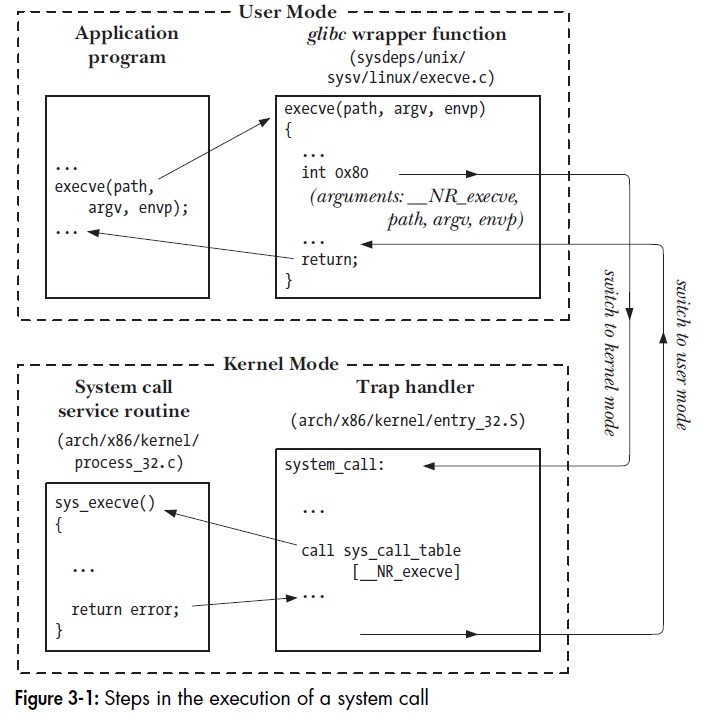
\includegraphics[width=13cm]{pics/syscall}}


\subsection{Classification of interrupts and exceptions}
\bit
\w \bb{interrupts}: asynchronously generated by H/W devices or timers
  \bit
  \w \bb{maskable interrupts}
  \w \bb{unmaskable interrupts}
  \eit
\w \bb{exceptions}: synchronously produced by the CPU while executing
   instructions 
  \bit
  \w \bb{faults}: something which can be corrected (e.g. page fault); \bb{eip}
  is saved and exception handler is executed, and then control is back to
  saved \bb{eip}
  \w \bb{traps}: reported immediately after execution of \bb{trapping
    instruction} 
  \w \bb{aborts}: some serious error
  \eit
\w \bb{programmed exceptions (a.k.a. software interrupts)}: ocurr at the
request of the programmer (e.g. \texttt{\textbf{int}} instruction)
\eit



\pagebreak
\section{File Systems}
Unix file sytem provides \bb{data files}, which are {\em uninterpreted byte
arrays\/} and \bb{directories}, which contain named references to data files
and other directories.

\subsection{Buffer cache}
 The buffer cache is a linked list of buf structures holding
 cached copies of disk block contents.  Caching disk blocks
 in memory reduces the number of disk reads and also provides
 a synchronization point for disk blocks used by multiple processes.

\paragraph{Interface}
\bit
\w To get a buffer for a particular disk block, call bread.
\w After changing buffer data, call bwrite to write it to disk.
\w When done with the buffer, call brelse.
\w Do not use the buffer after calling brelse.
\w Only one process at a time can use a buffer,
\w so do not keep them longer than necessary.
\eit
The implementation uses three state flags internally:
\bit
\w \verb+B_BUSY+: the block has been returned from bread
     and has not been passed back to brelse.  
\w \verb+B_VALID+: the buffer data has been read from the disk.
\w \verb+B_DIRTY+: the buffer data has been modified
     and needs to be written to disk.
\eit


\subsection{What happens when \texttt{fread} is executed?}
\bit
\w User calls \texttt{fread} in user space.
\begin{alltt}
  size_t fread(void *ptr, size_t size, size_t nmemb, FILE *stream);
\end{alltt}

\w Implementation of \texttt{fread} in LIBC calls read system call
\begin{alltt}
  ssize_t read(int fd, void *buf, size_t count);
\end{alltt}

\w Now, we're in kernel space.

\w \bb{SYSCALL.C}:\  \texttt{syscall()} is executed
  \begin{alltt}
  void \textbf{syscall}(void)
  \{
    int num;

    num = proc->tf->eax;
    if (num > 0 && num < NELEM(syscalls) && syscalls[num]) \{
      proc->tf->eax = \textcolor{red2}{\textbf{syscalls[num]()}};
    \} else \{
      ERROR(unknown\_syscall);
      proc->tf->eax = -1;
    \}
  \}
  \end{alltt}

\w \bb{SYSFILE.C}:\  \texttt{sys\_read()} is executed
\begin{alltt}
  \textbf{int sys_read(void)}
  \{
    struct file *f;
    int n;
    char *p;

    if (argfd(0, 0, &f) < 0 || argint(2, &n) < 0 || argptr(1, &p, n) < 0)
      return -1;
    return \textcolor{red2}{\textbf{fileread(f, p, n)}};
  \}
\end{alltt}

\w \bb{FILE.C}:\ \texttt{fileread()} is executed
  \begin{alltt}
  \textbf{int fileread(struct file *f, char *addr, int n)} 
  \{
    if (f->type == FD_PIPE) \{
      return piperead(f->pipe, addr, n);
    \}

    if (f->type == FD_INODE) \{
      \textcolor{red2}{\textbf{ilock(f->ip)}};
      if ((r = \textcolor{red2}{\textbf{readi(fp->ip, addr, f->off, n)}}) > 0)
        f->off += r;
      \textcolor{red2}{\textbf{iunlock(f->ip)}};
      return r;
    \}
  \}
  \end{alltt}

\w \bb{FS.C}:\ Read from the file system with \texttt{readi()}. 
  \begin{alltt}
  \textbf{int readi(struct inode *ip, char *dst, uint off, uint n)} 
  \{
    uint tot, m;
    struct buf *bp;

    if(ip->type == T_DEV) \{
      if(ip->major < 0 || ip->major >= NDEV || !devsw[ip->major].read)
        return -1;
      return \textcolor{red2}{\textbf{devsw[ip->major].read(ip, dst, n)}};
    \}

    if(off > ip->size || off + n < off)
      return -1;
    if(off + n > ip->size)
      n = ip->size - off;

    for (tot=0; tot<n; tot+=m, off+=m, dst+=m) \{
      bp = \textcolor{red2}{\textbf{bread(ip->dev, bmap(ip, off/BSIZE))}};
      m = min(n - tot, BSIZE - off%BSIZE);
      memmove(dst, bp->data + off%BSIZE, m);
      \textcolor{red2}{\textbf{brelse(bp)}};
    \}
    return n;
  \}
  \end{alltt}

\w \bb{BIO.C}:\ Read from buffer cache with \texttt{bread}
  \begin{alltt}
  \textbf{struct buf *bread(uint dev, uint sector)}
  \{
    struct buf *b;

    b = \textcolor{red2}{\textbf{bget(dev, sector)}};
    if(!(b->flags & B_VALID))
      \textcolor{red2}{\textbf{iderw(b)}};
    return b;
  \}
  \end{alltt}

\w \bb{IDE.C}:\ Simple PIO-based (non-DMA) 
                   \textcolor{red2}{\textbf{IDE device driver}}

  \begin{alltt}
  \textbf{void iderw(struct buf *b)}
  \{
    struct buf **pp;

    if (!(b->flags & B_BUSY))
      panic("iderw: buf not busy");
    if ((b->flags & (B_VALID|B_DIRTY)) == B_VALID)
      panic("iderw: nothing to do");
    if (b->dev != 0 && !havedisk1)
      panic("iderw: ide disk 1 not present");

    \textbf{acquire(&idelock)};

    // Append b to idequeue.
    b->qnext = 0;
    for (pp=&idequeue; *pp; pp=&(*pp)->qnext)
      ;
    *pp = b;
  
    // Start disk if necessary.
    if(idequeue == b)
      \textcolor{red2}{\textbf{idestart(b)}};
  
    // Wait for request to finish.
    while((b->flags & (B_VALID|B_DIRTY)) != B_VALID) \{
      sleep(b, &idelock);
    \}
    \textbf{release(&idelock)};
  \}
  \end{alltt}
\eit


\pagebreak
\section{X86 Assembly Tutorial}
For more detailed information about the architecture and about processor
instructions, you will need access to a 486 (or 386) microprocessor
manual. For more details, see The 80386 book, by Ross P. Nelson.
Intel
processor manuals may also be found at
http://www.x86.org/intel.doc/586manuals.htm. 

The GNU Assembler, gas, uses a different syntax from what you will likely find in any x86 reference manual, and the two-operand instructions have the source and destinations in the opposite order. Here are the types of the gas instructions:
\begin{verbatim}
    opcode                    (e.g., pushal)
    opcode operand            (e.g., pushl %edx)
    opcode source,dest        (e.g., movl %edx,%eax) (e.g., addl %edx,%eax)
\end{verbatim}
Where there are two operands, the rightmost one is the destination. The leftmost one is the source. 
For example, \verb+movl %edx, %eax+ means Move the contents of the edx
register into the eax register. For another example,
                        \verb+addl %edx,%eax+ means Add the contents of the edx and
                        eax registers, and place the sum in the eax
                        register. 

Included in the syntactic differences between gas and Intel assemblers is that
all register names used as operands must be preceeded by a percent (\verb+%+)
                                sign, and instruction names usually end in
                                either "l", "w", or "b", indicating the size
                                of the operands: long (32 bits), word (16
                                bits), or byte (8 bits), respectively. For
                                our purposes, we will usually be using the
                                "l" (long) suffix. 

\subsection{80386+ Register Set}
There are different names for the same register depending on what part of the register you want to use. To use the first set of 8 bits of eax (bits 0-7), you would use %al. For the second set of 8 bits (bits 8-15) of eax you would use %ah. To refer to the lowest 16 bits of eax (bits 0-15) together you would use %ax. For the entire 32 bits you would use %eax (90% of the time this is what you will be using). The form of the register name must agree with the size suffix of the instruction.

Here are the important processor registers:
\begin{verbatim}
    EAX,EBX,ECX,EDX - "general purpose", more or less interchangeable

    EBP             - used to access data on stack
                    - when this register is used to specify an address, SS is
                      used implicitly

    ESI,EDI         - index registers, relative to DS,ES respectively

    SS,DS,CS,ES,FS,GS - segment registers
                      - (when Intel went from the 286 to the 386, they figured
                         that providing more segment registers would be more
                         useful to programmers than providing more general-
                         purpose registers... now, they have an essentially
                         RISC processor with only _FOUR_ GPRs!)
                      - these are all only 16 bits in size

    EIP            - program counter (instruction pointer), relative to CS

    ESP            - stack pointer, relative to SS

    EFLAGS         - condition codes, a.k.a. flags
\end{verbatim}

\subsection{Segmentation}
We are using the 32-bit segment addressing feature of the 486. Using 32-bit addressing as opposed to 16-bit addressing gives us many advantages:
No need to worry about 64K segments. Segments can be 4 gigabytes in length under the 32-bit architecture.
32-bit segments have a protection mechanism for segments, which you have the option of using.
You don't have to deal with any of that ugly 16-bit crud that is used in other operating systems for the PC, like DOS or OS/2; 32-bit segmentation is really a thing of beauty in comparison to that.
i486 addresses are formed from a segment base address plus an offset. To compute an absolute memory address, the i486 figures out which segment register is being used, and uses the value in that segment register as an index into the global descriptor table (GDT). The entry in the GDT tells (among other things) what the absolute address of the start of the segment is. The processor takes this base address and adds on the offset to come up with the final absolute address for an operation. You'll be able to look in a 486 manual for more information about this or about the GDT's organization.

i486 has 6 16-bit segment registers, listed here in order of importance:
\ben
\w \bb{CS (Code Segment Register):}
Added to address during instruction fetch.
\w \bb{SS (Stack Segment Register)}:
Added to address during stack access.
\w \bb{DS (Data Segment Register)}:
Added to address when accessing a memory operand that is not on the stack.
\w \bb{ES, FS, GS (Extra Segment Registers)}:
Can be used as extra segment registers; also used in special instructions that
span segments (like string copies).
\een
The x86 architecture supports different addressing modes for the operands. A discussion of all modes is out of the scope of this tutorial, and you may refer to your favorite x86 reference manual for a painfully-detailed discussion of them. Segment registers are special, you can't do a
\begin{verbatim}
    movw seg-reg, seg-reg
\end{verbatim}
You can, however, do
\begin{verbatim}
    movw seg-reg,memory
    movw memory,seg-reg
    movw seg-reg,reg
    movw reg,seg-reg
\end{verbatim}
Note: If you \verb+movw %ss,%ax+, then you should \verb+xorl %eax,%eax+ first to clear the high-order 16 bits of eax, so you can work with long values.
 
\subsection{Common/Useful Instructions}
\begin{verbatim}
mov (especially with segment registers)
    - e.g.,:
        movw %es,%ax
        movl %cs:4,%esp
        movw _processControlBlock,%cs

    - note:     mov's do NOT set flags

pushl, popl       - push/pop long
pushal, popal     - push/pop EAX,EBX,ECX,EDX,ESP,EBP,ESI,EDI

call  (jumps to piece of code, saves return address on stack)
         e.g., call _cFunction

int   - call a software interrupt

ret   (returns from piece of code entered due to call instruction)
iretl (returns from piece of code entered due to hardware or software interrupt)

sti, cli - set/clear the interrupt bit to enable/disable interrupts respectively
lea  - is Load Effective Address, it's basically a direct pipeline to the
       address you want to do calculations on without affecting any flags, 
       or the need of pushing and popping flags. 
\end{verbatim}
\subsection{A simple example}
\begin{verbatim}
CODE
void funtction1() {
	int A = 10;
	A += 66;
}

compiles to...
funtction1:
1	pushl %ebp #
2	movl %esp, %ebp #,
3	subl $4, %esp #,
4	movl $10, -4(%ebp) #, A
5	leal -4(%ebp), %eax #, 
6	addl $66, (%eax) #, A
7	leave
8	ret
\end{verbatim}
Explanation:
\ben
\w push ebp
\w  copy stack pointer to ebp
\w  make space on stack for local data
\w put value 10 in A (this would be the address A has now)
\w load address of A into EAX (similar to a pointer)
\w add 66 to A
\een
... don't think you need to know the rest

\subsection{Mixing C and Assembly Language}
The way to mix C and assembly language is to use the "asm" directive. To
access C-language variables from inside of assembly language, you simply use
the C identifier name as a memory operand. These variables cannot be local to
a procedure, and also cannot be static inside a procedure. They must be global
(but can be static global). The newline characters are necessary. 

\begin{verbatim}
unsigned long a1, r;
void junk( void )
{
   asm(
        "pushl %eax \n"
        "pushl %ebx \n"
        "movl $100,%eax \n"
        "movl a1,%ebx \n"
        "int $69 \n"
        "movl %eax,r \n"
        "popl %ebx \n"
        "popl %eax \n"
   );
}
\end{verbatim}
This example does the following:
\ben
\w Pushes the value stored in eax and ebx onto the stack.
\w  Puts a value of 100 into eax.
\w  Copies the value in global variable a1 into ebx.
\w  Executes a software interrupt number 69.
\w  Copies the value in eax into the global variable r.
\w  Restores (pops) the contents of the temporary registers eax and ebx.
\een

\section{JOS Virtual Memory Map}
\centerline{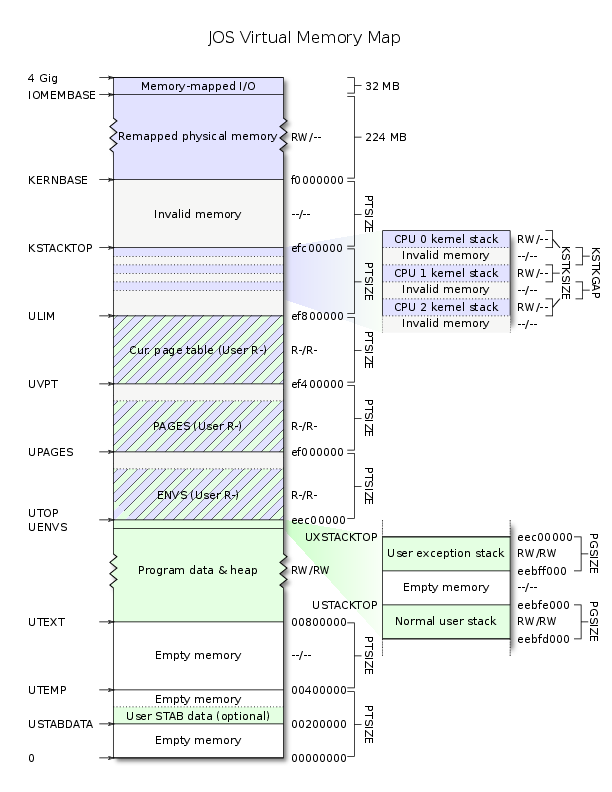
\includegraphics[width=13cm]{pics/jos_layout}}

\end{document}

